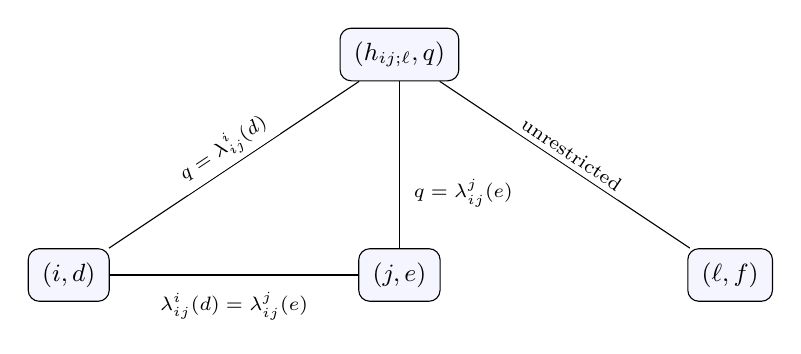
\begin{tikzpicture}[
  vertex/.style={draw,rounded corners,fill=blue!4,inner sep=5pt},
  every node/.style={font=\small},
  test/.style={font=\scriptsize,fill=white,inner sep=2pt}
]
\node[vertex] (left) at (-4.2,0) {\((i,d)\)};
\node[vertex] (middle) at (0,0) {\((j,e)\)};
\node[vertex] (right) at (4.2,0) {\((\ell,f)\)};
\node[vertex] (helper) at (0,2.8) {\((h_{ij;\ell},q)\)};
\draw (helper) -- node[test,sloped,above] {\(q=\lambda_{ij}^i(d)\)} (left);
\draw (helper) -- node[test,pos=.67,right=3pt] {\(q=\lambda_{ij}^j(e)\)} (middle);
\draw (helper) -- node[test,sloped,above] {unrestricted} (right);
\draw (left) -- node[test,below=4pt] {\(\lambda_{ij}^i(d)=\lambda_{ij}^j(e)\)} (middle);
\end{tikzpicture}
